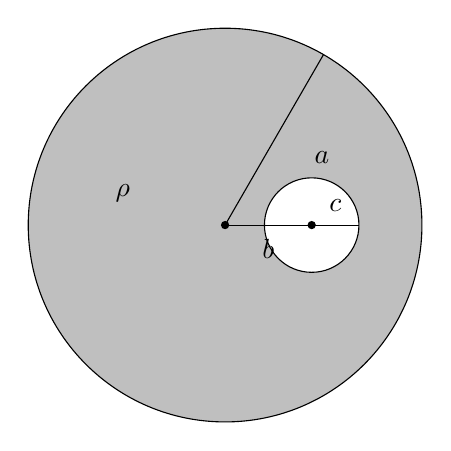
\begin{tikzpicture}
% big disk
\fill[gray!50] (0,0) circle (2.5);
% hole
\fill[white] (1.1,0) circle (0.6);
\draw (0,0) circle (2.5);
\draw (1.1,0) circle (0.6);
% centers
\fill (0,0) circle (1.5pt);
\fill (1.1,0) circle (1.5pt);
% radius a to outer edge
\draw (0,0) -- (60:2.5);
\node at (35:1.5) {$a$};
% b to hole center
\draw (0,0) -- (1.1,0);
\node[below] at (0.55,-0.05){$b$};
% c hole radius
\draw (1.1,0) -- (1.7,0);
\node[above] at (1.4,0.05){$c$};
% rho
\node at (-1.3,0.4){$\rho$};
\end{tikzpicture}
